\chapter{Introduction} % Main chapter title
\label{Chapter1}

\epigraph{Turbulence is the most important unsolved problem of classical physics.}{\textit{Richard Feynman}}

Turbulent flows have long been a phenomenon that is surprisingly easy to detect and observe in the natural world but unmistakably challenging to understand and model in sufficient detail, unlike other problems in classical physics.
The fundamental aspects of turbulent flow consisting of eddies of various length scales had long been observed, as recorded by Leonardo Da Vinci's $16^{th}$ century diagrams of water flow in streams and channels from the  \parencite{Colagrossi2021DaVinci}.
It took the work of Osborne Reynolds and William Thomson (Lord Kelvin) from the late $19th$ century for the scientific community to demarcate the separation between the laminar and turbulent flow. However, further strides in the field have remained arduous despite the Navier-Stokes (NS) equations being written down in the early $19^{th}$ century. There is consensus that this remarkable failure of some of the greatest scientific minds in providing an intricate understanding of turbulence points to an inadequacy of the mathematical tools we have at our disposal. Even the current machinery cannot deal with the strong non-linearity of the equations coupled with the characteristic tendency of flows to degenerate into some form of instability.

\begin{figure}[h!]
    \centering
    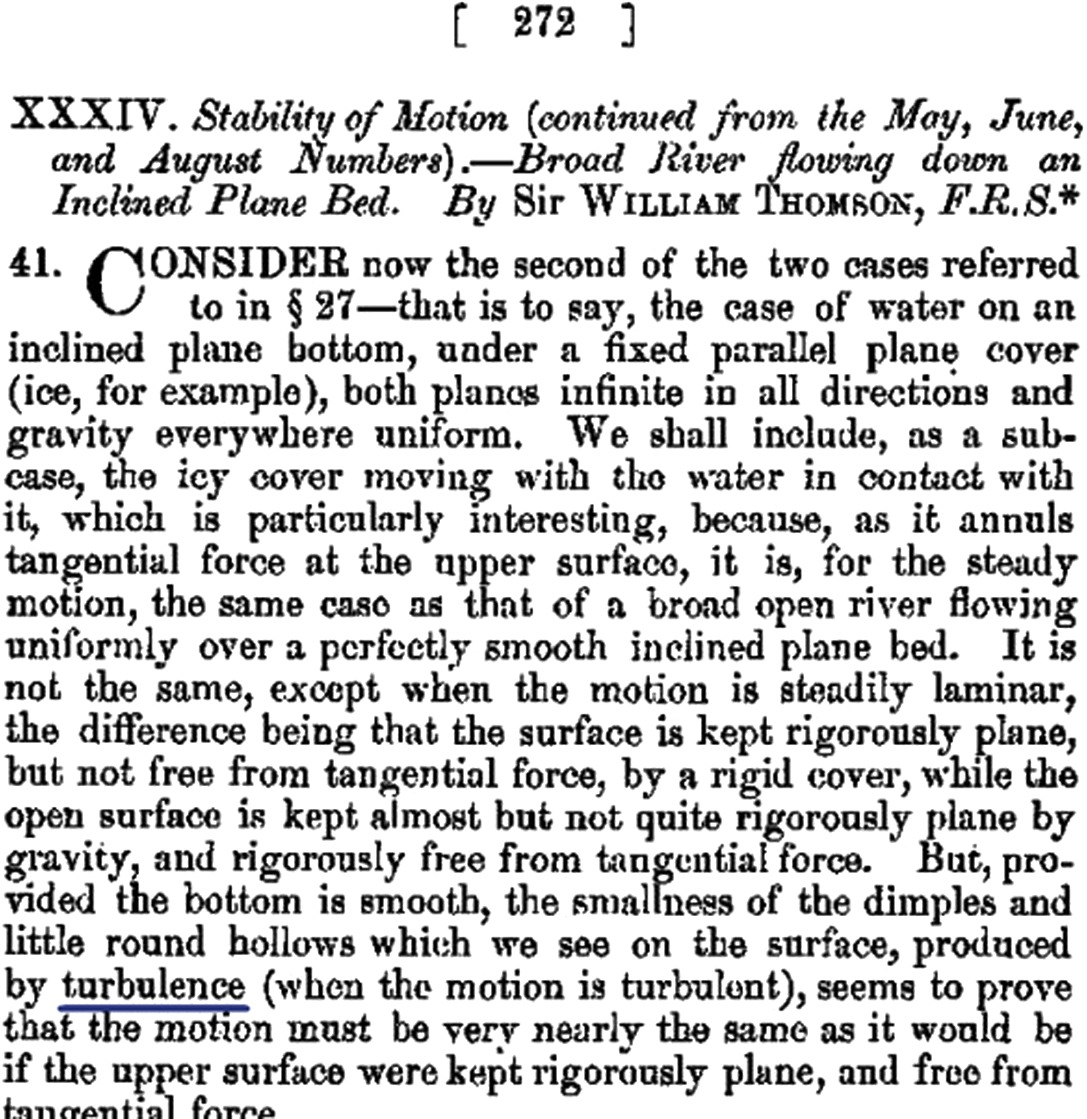
\includegraphics{Figures/research_papers/schmitt2017turbulence-fig-1.jpg}
    \caption{A scanned copy of a part of the first page of the 1887 paper by William Thomson, where the word \textit{'turbulence'}, as a noun, is first introduced. Ref: \parencite{schmitt2017turbulence}}
    \label{fig:schmitt2017turbulence-fig-1}
\end{figure}

Turbulence is caused by excessive kinetic energy in parts of a fluid flow that can overcome the damping effect of the fluid's viscosity. Its onset can be predicted by the dimensionless Reynolds number, which is the ratio of kinetic energy to viscous damping in a fluid flow. 

The criteria for defining a flow as turbulent are varied and ambiguous since there is no explicit definition for it. However, the most often used criteria for qualifying a flow as turbulent is given below \parencite{sagaut2002statistical}:
\begin{itemize}
    \item random character of the spatial and temporal fluctuations of the velocities, which reflect the existence of finite characteristic scales of statistical correlation;
    \item velocity field is three-dimensional and rotational;
    \item various modes are strongly coupled, which is reflected in the non-linearity of the NS equations;
    \item large mixing capacity due to the agitation induced by the various scales;
    \item chaotic character of the solution, which exhibits a powerful dependency on the initial condition and boundary conditions.
\end{itemize}

\section{Smoothed Particle Hydrodynamics}
Smoothed particle hydrodynamics (SPH) is a technique for problem-solving in \textit{Computational Continuum Dynamics} (CCD). This technique approximates numerical solutions of the equations of fluid dynamics by replacing the fluid with a set of particles. The equations of motion and properties of these particles are determined from the continuum equations of fluid dynamics. They are subsequently discretised based on the particles' interpolant data. The interpolant can be constructed using analytical functions, and spatial derivatives of the interpolated quantities can then be found using ordinary calculus. There is no need to use a grid, and the description of free surfaces, however complicated, is trivial.

Therefore, this \textit{Lagrangian} based particle formulation uses no background spatial mesh. Since there is no mesh to distort, the method can handle large deformations in a pure Lagrangian frame. Thus, material interfaces can be modelled naturally, and complex constitutive behaviour can be implemented relatively quickly. This allows SPH to have diverse and fascinating applications in various domains that extend beyond the astrophysical and cosmological problems it was initially designed to tackle.

\section{Project Motivation \& Objectives}
Despite the success of SPH in simulating transient flows, a robust or rigorous model of turbulence does not seem to exist. Some of the models in use cannot be generalised to a wide variety of turbulence-based problems or scaled to $3D$-flows.
This limits SPH's applicability in turbulent flows where conventional FEM/FVM-based CFD solvers have the upper hand, owing to their sophisticated models.

This project aims to survey and review the current state of the art regarding turbulence modelling in SPH and subsequently provide a framework to help establish the advantages and limitations of such models, using a comparative analysis between the major class of models.
After that, it is intended to extend the most well-equipped models to robust and accurate SPH schemes (which might not have been the case in the author/s original work). Such an exercise is expected to either improve the original model or expose any underlying limitations in its assumptions or discretisation.

\section{Report Structure}
The report is structured to present the turbulence models developed for SPH in Chapter \ref{Chapter2}. Here, the models have been categorised by the fundamental ideas on which they were based. Subsequently, research on analysing turbulence through standard benchmarks problems and methods of quantifying turbulence data is presented in Chapter \ref{Chapter3}.
Finally, the project conclusion and future work for Stage - II of the Dual Degree Project are presented in Chapter \ref{Chapter4}. 
